\documentclass[border=10pt]{standalone}
\usepackage{tikz}
\usetikzlibrary{arrows.meta, shapes, calc}

\begin{document}
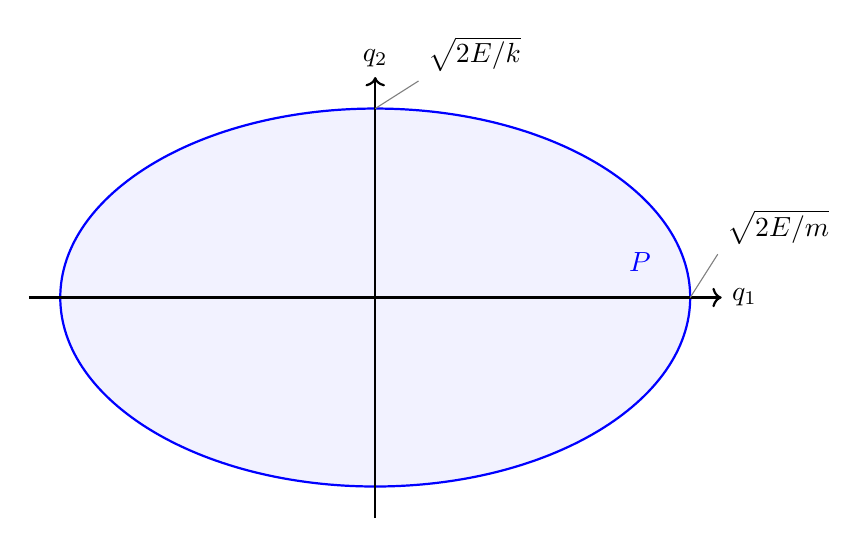
\begin{tikzpicture}
    % Shade the ellipse
    \fill[blue!5] (0,0) ellipse (4cm and 2.4cm);

    % Draw the ellipse
    \draw[thick, blue] (0,0) ellipse (4cm and 2.4cm);
    
    % Draw the coordinate axes
    \draw[thick,->] (-4.4,0) -- (4.4,0) node[right] {$q_1$};
    \draw[thick,->] (0,-2.8) -- (0,2.8) node[above] {$q_2$};
    
    % Label the intersection points
    \draw[thin, gray] (4,0) -- (4.35,0.55);
    \node at (4.35,0.55) [above right] {$\sqrt{2E/m}$};
    \draw[thin, gray] (0,2.4) -- (0.55,2.75);
    \node at (0.55,2.75) [above right] {$\sqrt{2E/k}$};
    
    % Label the point P
    \node[blue] at (3.1,0.45) [right] {$P$};
\end{tikzpicture}
\end{document}
